\section{Results}
\fxnote{This should be a collaborative section}

\subsection{\label{sec:gridstudy}Domain and grid resolution study}

In order to ensure that the large and small turbulence scales were
properly resolved in the offshore LES simulations, the appropriate
domain size and mesh resolution needed to be determined.
Under-resolved meshes or domain sizes which are too small may miss the
smaller turbulence scales or remove the larger structures required for
proper ABL development.  However, over-resolved meshes or
unnecessarily large domains might lead to excessive computational
requirements to complete the simulations.

The appopriateness of these meshes and domain sizes were determined
based on wind spectra and integral length scale they were able to capture.

The maximum resolvable frequency on a mesh with grid size $\Delta$ and
average horizontal wind speed $\bar{U}_{horiz}$ can be estimated as
\begin{equation}
  \label{eq:fmax}
  f_{max} = \frac{0.6\bar{U}_{horiz}}{N\Delta}.
\end{equation}
Here, equation \ref{eq:fmax} assumes that the turbulent eddies convect
with a velocity of $0.6\bar{U}_{horiz}$ and $N=8$ is chosen for the
purposes of this study.  Due to the alignment of the flow with the
mesh directions, the grid size $\Delta = \sqrt{2}\cdot \textrm{dx}$.

%%%%%%%%%%%%%%% GRID STUDY: INTEGRAL LENGTH %%%%%%%%%%%%%%%%%%%%%%%%
\begin{table}
\caption{\label{tab:GridStudySetup} The setup for the grid resolution study} \centering
\begin{tabular}{ccccc}
  \hline
  Case              & dx [m] & dy [m] & dz [m] & Domain size \\
  \hline
  Nalu-wind coarse  &  10.0  & 10.0   & 2.5 & 1.5km x 1.5km x 1.0km  \\
  Nalu-wind medium  &   5.0  &  5.0   & 2.5 & 1.5km x 1.5km x 1.0km  \\
  Nalu-wind fine    &   2.5  &  2.5   & 2.5 & 0.0 \\
  AMR-wind fine     &   2.5  &  2.5   & 2.5 & 0.0 \\
\hline
\end{tabular}
\end{table}
%%%%%%%%%%%%%%%%%%%%%%%%%%%%%%%%%%%%%%%%%%%%%%%%%%%%%%%%%%%%%%%%%%%%

The wind spectra
\begin{equation}
  \int_0^\infty S_i(f) \textrm{d}f = \sigma_i^2
\end{equation}

%%%%%%%%%%% Grid resolution spectra figure %%%%%%%%%%%%%%%%%%%%%%%%%
% Created in Postprocessing/GridStudy/GridStudy_Spectra.ipynb
\begin{figure}[hbt!]
  \label{fig:GridStudySpectra}
  \centering
  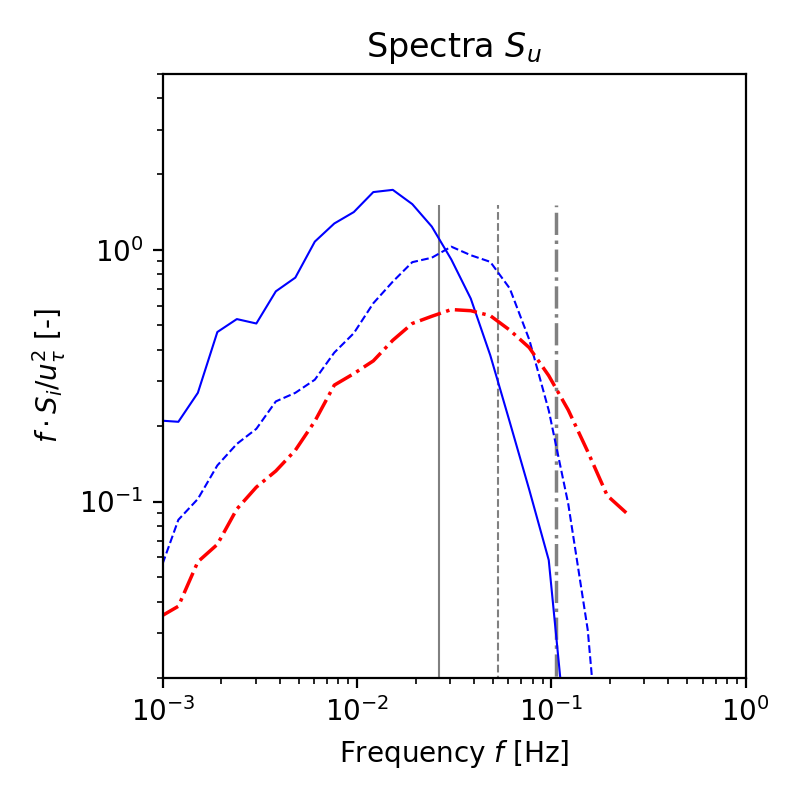
\includegraphics[width=2.0in]{figures/GridStudy_Spectra_Su.png}
  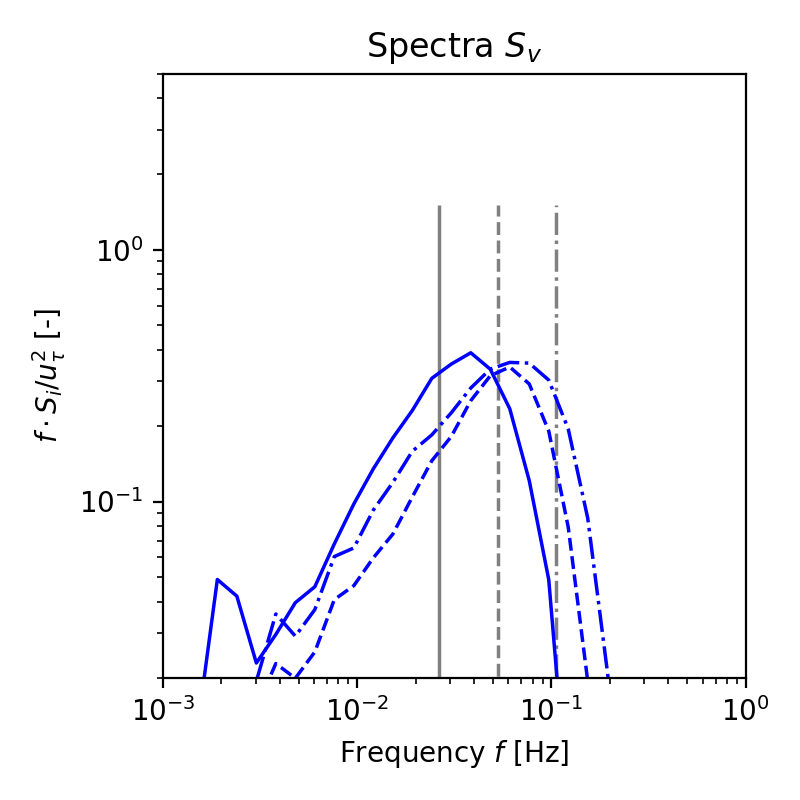
\includegraphics[width=2.0in]{figures/GridStudy_Spectra_Sv.png}
  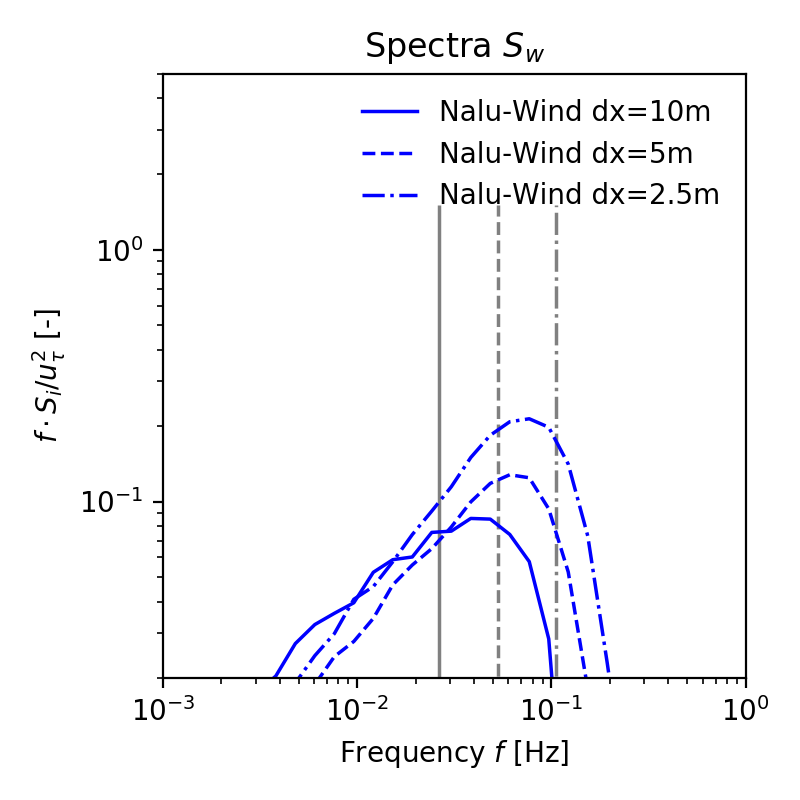
\includegraphics[width=2.0in]{figures/GridStudy_Spectra_Sw.png}
  \caption{Calculation of the wind spectra $S_i$ for LES of stable
    5m/s case with different resolutions.  The gray vertical lines
    correspond to the maximum resolvable frequency $f_{max}$ according
    to equation (\ref{eq:fmax}). }
\end{figure}
%%%%%%%%%%%%%%%%%%%%%%%%%%%%%%%%%%%%%%%%%%%%%%%%%%%%%%%%%%%%%%%%%%%%

The two-point correlation tensor defined as
\begin{equation}
  \label{eq:Rij}
  R_{ij}({\mathbf x},\boldsymbol{\xi}) = 
  \frac{\overline{ {u'_i(\mathbf{x}, t) u'_j(\mathbf{x}+\boldsymbol{\xi},t)} }}
       { \sqrt{\overline{ u'^2_i }} \sqrt{\overline{ u'^2_j}} }
\end{equation}
where the velocity fluctuations $u'_i$ are defined as 
\begin{equation}
  u'_i(\mathbf{x},t) = u_i(\mathbf{x},t) - \overline{ u_i(\mathbf{x},t) }
\end{equation}

The horizontally averaged correlation coefficient $\langle
R_{ij}(\boldsymbol{\xi})\rangle$ is computed from
$R_{ij}(\mathbf{x},\boldsymbol{\xi})$ by sampling over ...

%%%%%%%%%%% Grid resolution Rij correlation figure %%%%%%%%%%%%%%%%%%%%
% Created in Postprocessing/GridStudy/GridStudy_Rij.ipynb
\begin{figure}[hbt!]
  \label{fig:GridStudyRij}
  \centering
  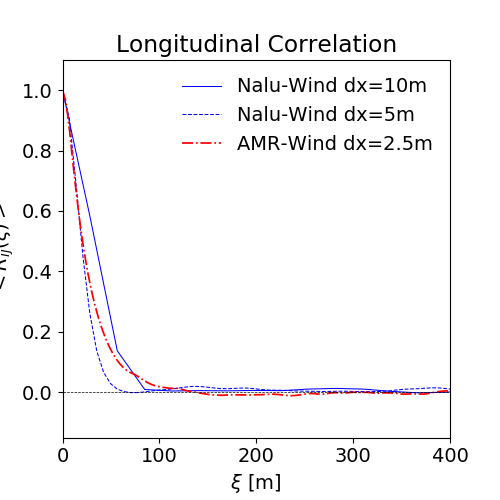
\includegraphics[width=3in]{figures/GridStudy_Rij_Longitudinal.png}
  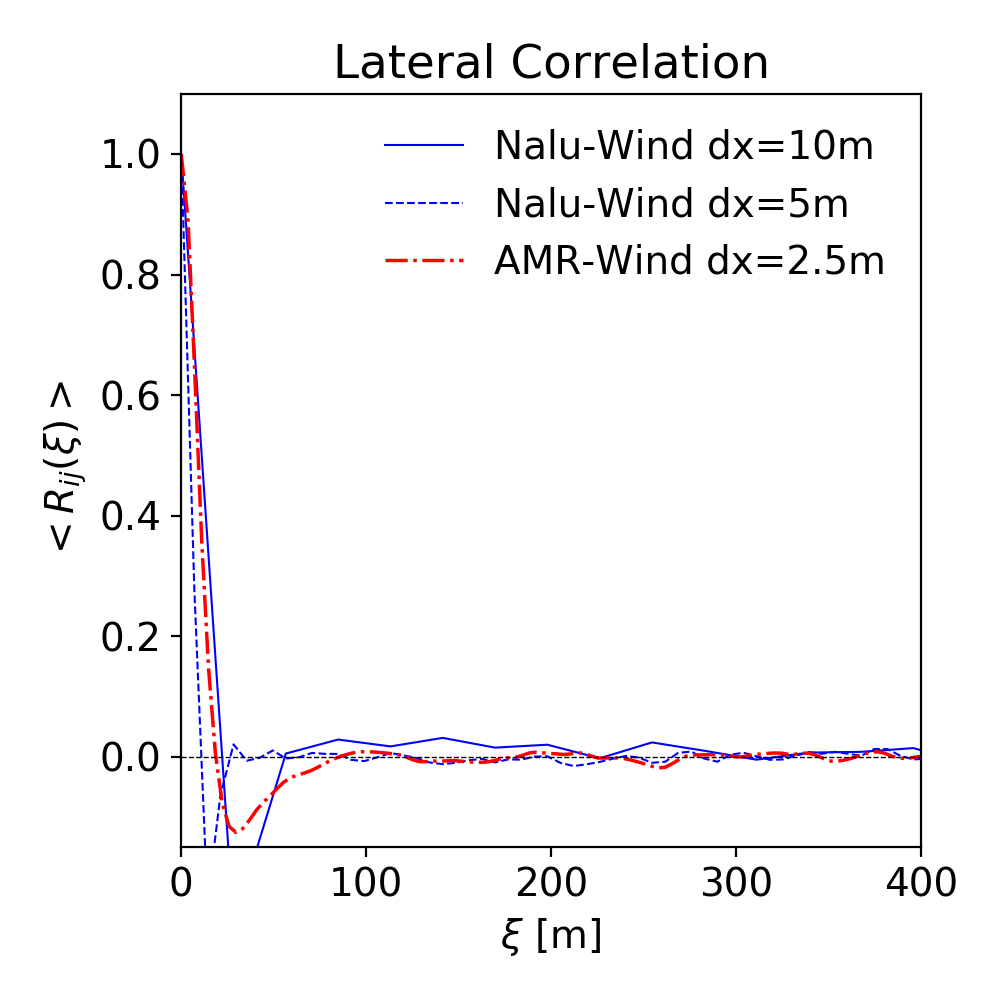
\includegraphics[width=3in]{figures/GridStudy_Rij_Lateral.png}
  \caption{Calculation of the averaged longitudinal and lateral
    $R_{ij}(\xi)$ coefficient at $z$=20m for LES of stable 5m/s case
    with different resolutions.}
\end{figure}
%%%%%%%%%%%%%%%%%%%%%%%%%%%%%%%%%%%%%%%%%%%%%%%%%%%%%%%%%%%%%%%%%%%%


The turbulent integral lengthscale can be calculated from $\langle
R_{ij}(\xi) \rangle$ via
\begin{equation}
  L = \int_0^\infty \langle R_{ij}(\xi) \rangle \: {\textrm d}\xi
\end{equation}

%%%%%%%%%%%%%%% GRID STUDY: INTEGRAL LENGTH %%%%%%%%%%%%%%%%%%%%%%%%%%%%%%%%%%%
\begin{table}
\caption{\label{tab:GridStudyLscale} The calculated turbulent integral
  lengthscale for each of the grid resolutions} \centering
\begin{tabular}{ccccc}
  \hline
  Case              & dx [m] & Longitudinal L [m] & Lateral L [m] \\
  \hline
  Nalu-wind coarse  &  10.0  & 36.433999          & 0.0        \\
  Nalu-wind medium  &   5.0  & 21.485711          & 4.519247   \\
  Nalu-wind fine    &   2.5  & 25.250568          & 5.919645   \\
  AMR-wind fine     &   2.5  & 27.689340          & 9.332672   \\
\hline
\end{tabular}
\end{table}

\subsection{Comparison of AMR-Wind vs Nalu-Wind}
\fxnote{COMPARE AMR-WIND VS NALU-WIND HERE}

%%%%%%%%%%%%%%% Compare Nalu/AMR integrated quantities %%%%%%%%%%%%%%
\begin{table}
\caption{\label{tab:CompareAMRvsNalu} Comparison of AMR-Wind and Nalu-Wind} \centering
\begin{tabular}{ccccc}
  \hline
  Case          & TI        &  $\alpha$  &   $u_\tau$ &       L \\
  \hline
  naluwind 5m/s &  0.048106 &  0.165277 &  0.163342 & 94.970836 \\
  amrwind 5m/s  &  0.048255 &  0.165552 &  0.157399 & 52.512434 \\
  \hline
\end{tabular}
\end{table}
%%%%%%%%%%%%%%%%%%%%%%%%%%%%%%%%%%%%%%%%%%%%%%%%%%%%%%%%%%%%%%%%%%%%

%%%%%%%%%%% Compare Nalu/AMR profiles %%%%%%%%%%%%%%%%%%%%%%%%%%%%%%
% AMRWind_NaluWind_stable_05ms_mesh2_5x2_5x2_5.ipynb
\begin{figure}[hbt!]
  \label{fig:CompareAMRvsNaluProfiles}
  \centering
  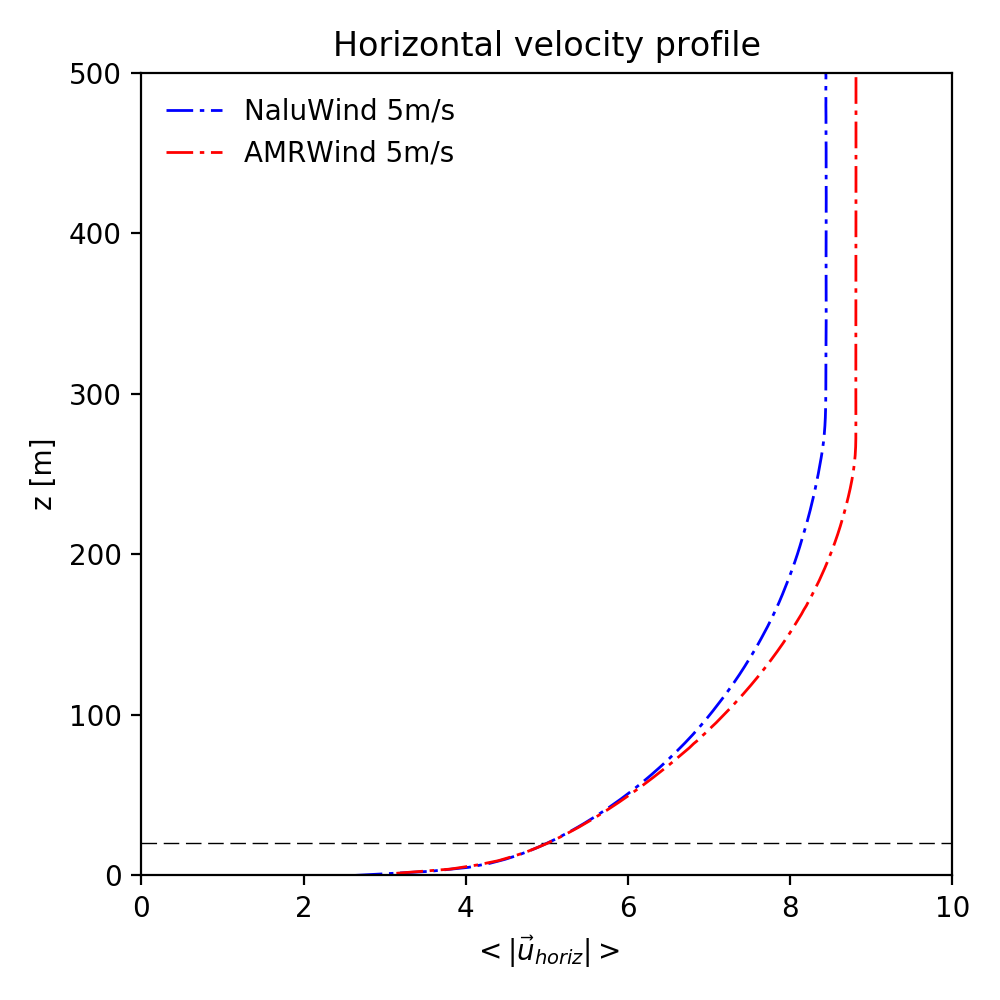
\includegraphics[width=6.0in]{figures/Compare_AMRWind_NaluWind/AMRWind_NaluWind_stable_05ms_mesh2p5_2p5_2p5_WS.png}\\
  \includegraphics[width=6.0in]{figures/Compare_AMRWind_NaluWind/AMRWind_NaluWind_stable_05ms_mesh2p5_2p5_2p5_Wdir.png}\\
  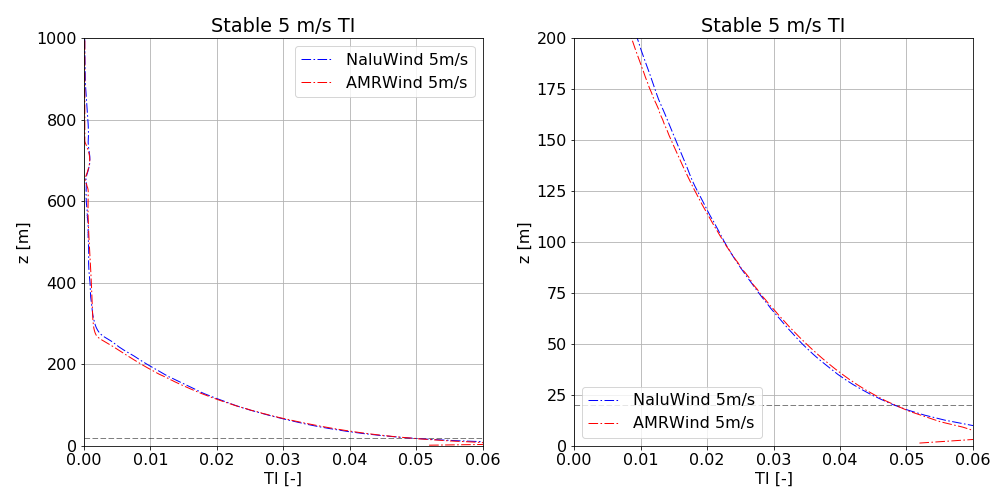
\includegraphics[width=6.0in]{figures/Compare_AMRWind_NaluWind/AMRWind_NaluWind_stable_05ms_mesh2p5_2p5_2p5_TI.png}
  \caption{Comparison of AMR-Wind and Nalu-Wind profiles. }
\end{figure}
%%%%%%%%%%%%%%%%%%%%%%%%%%%%%%%%%%%%%%%%%%%%%%%%%%%%%%%%%%%%%%%%%%%%

%%%%%%%%%%% Compare Nalu/AMR spectra %%%%%%%%%%%%%%%%%%%%%%%%%%%%%%%%
% Postprocessing/ABLSpectra/AMRWind_NaluWind_Spectra_Stable.ipynb
\begin{figure}[hbt!]
  \label{fig:CompareAMRvsNaluSpectra}
  \centering
  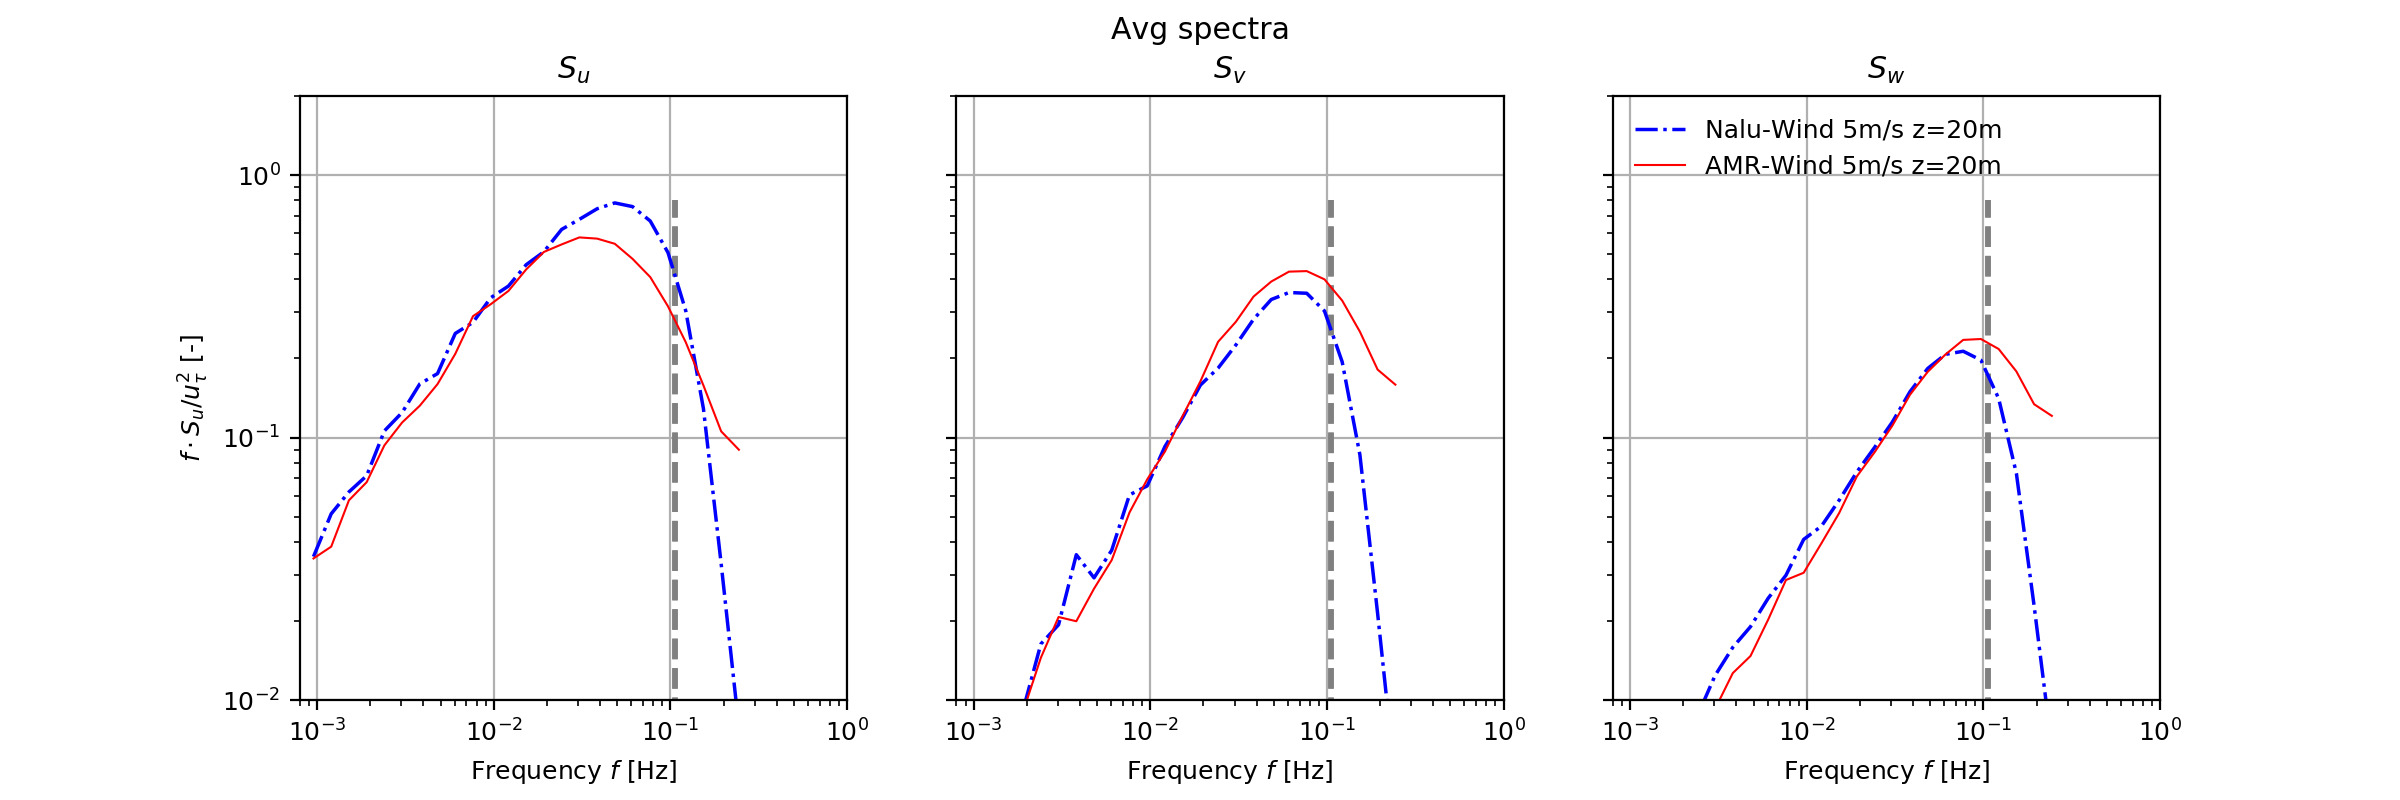
\includegraphics[width=6.0in]{figures/Compare_AMRWind_NaluWind/AMRWind_NaluWind_Spectra_Stable_z20.png}

  \caption{Comparison of AMR-Wind and Nalu-Wind wind spectra at
    z=20m. }
\end{figure}
%%%%%%%%%%%%%%%%%%%%%%%%%%%%%%%%%%%%%%%%%%%%%%%%%%%%%%%%%%%%%%%%%%%%

%%%%%%%%%%% Compare Nalu/AMR lengthscale %%%%%%%%%%%%%%%%%%%%%%%%%%%%
% Postprocessing/ABLLength/CompareAMRNalu_ABL_Lengthscales.ipynb
\begin{figure}[hbt!]
  \label{fig:CompareAMRvsNaluRij}
  \centering
  \fxnote{UPDATE THIS FIGURE}\\
  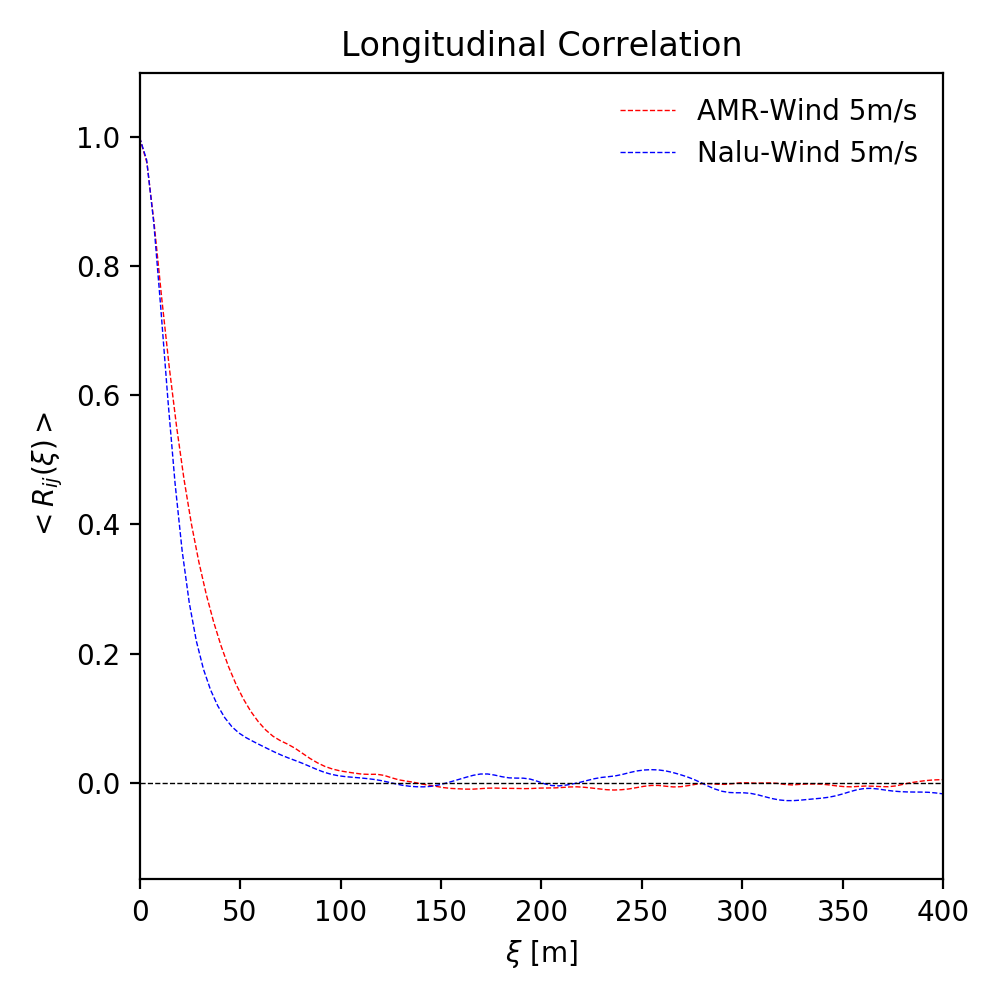
\includegraphics[width=2.5in]{figures/Compare_AMRWind_NaluWind/AMRWind_NaluWind_Lengthscale_Stable_z20_Longitudinal.png}
  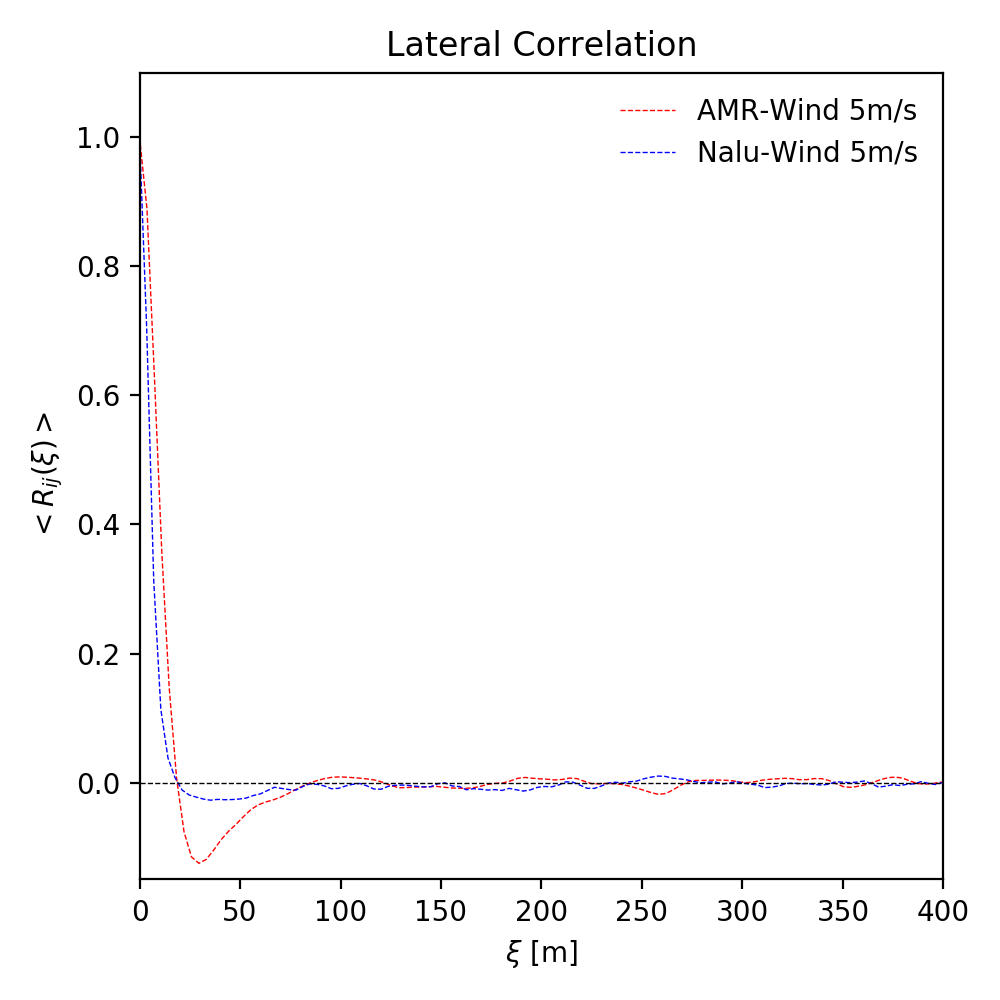
\includegraphics[width=2.5in]{figures/Compare_AMRWind_NaluWind/AMRWind_NaluWind_Lengthscale_Stable_z20_Lateral.png}

  \caption{Comparison of AMR-Wind and Nalu-Wind $\langle R_{ij}
    \rangle$ correlation at z=20m. }
\end{figure}
%%%%%%%%%%%%%%%%%%%%%%%%%%%%%%%%%%%%%%%%%%%%%%%%%%%%%%%%%%%%%%%%%%%%

\subsection{ABL Physics}

\subsubsection{ABL integrated quantities}
Describe integrated quantities

\subsubsection{Horizontally averaged profiles}

\subsubsection{Wind spectra and turbulence statistics}

The Kaimal model for spectra \cite{kaimal1973turbulence,
  cheynet2017spectral} for neutral atmospheric conditions:
\begin{equation}
  \label{eq:kaimal}
  \frac{fS_i}{u_\tau^2} = \frac{a_i(fz/\bar{U})}{\left(1+b_i(fz/\bar{U})^{\alpha_i}\right)^{\beta_i}}
\end{equation}

%%%%%%%%%%%%%%% KAIMAL MODEL PARAMETERS %%%%%%%%%%%%%%%%%%%%%%%%%%%%%%%%%%%
\begin{table}
\caption{\label{tab:KaimalParameters} Parameters for Kaimal model}
\centering
\begin{tabular}{ccccc}
  \hline
  Velocity & $a_i$ & $b_i$ & $\alpha_i$  & $\beta_i$ \\
  \hline
  $u$      & 105.0 & 33.0  & 1           & 5/3  \\
  $v$      &  17.0 &  9.5  & 1           & 5/3  \\
  $w$      &   2.1 &  5.3  & 5/3         &   1  \\
\hline
\end{tabular}
\end{table}


%%%%%%%%%%% Grid resolution spectra figure %%%%%%%%%%%%%%%%%%%%%%%%%
% Created in Postprocessing/ABLSpectra/Stable_Spectra_Allz.ipynb
\begin{figure}[hbt!]
  \label{fig:ABLSpectra_AllZ}
  \centering
  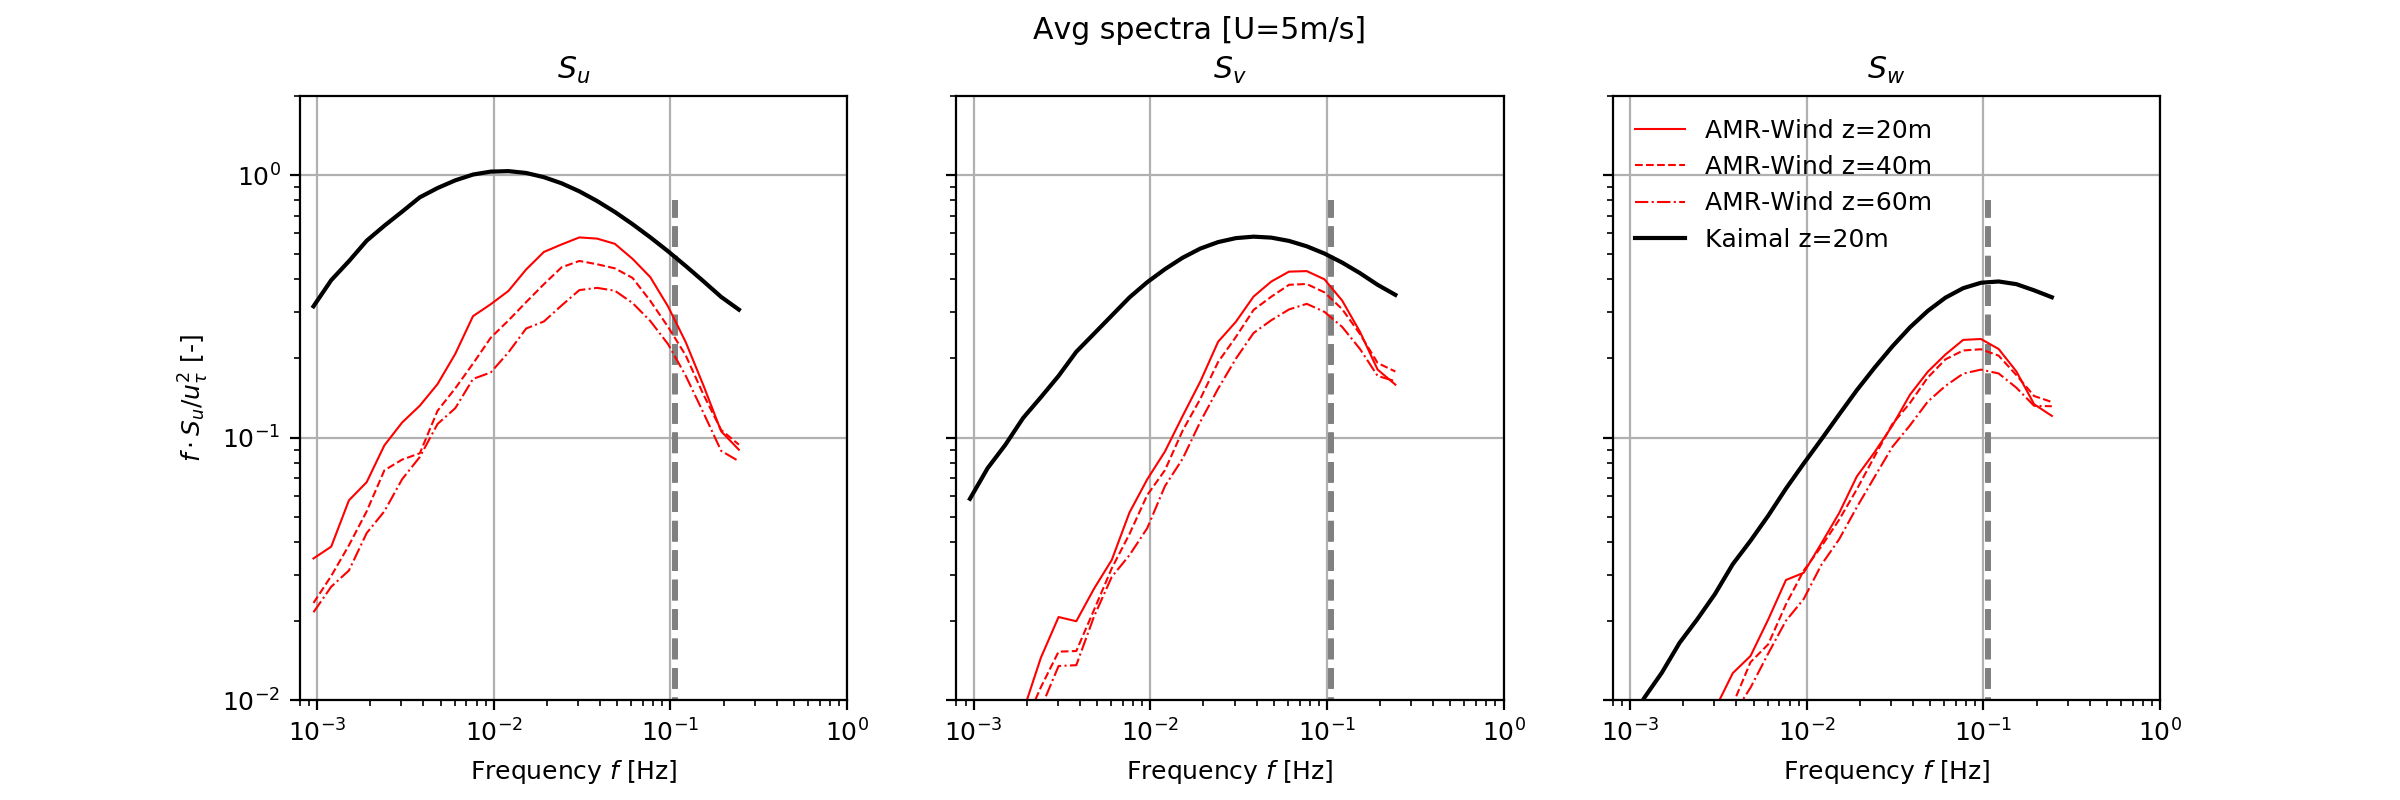
\includegraphics[width=7.0in]{figures/Stable_Spectra_AllZ_05ms.png}\\
  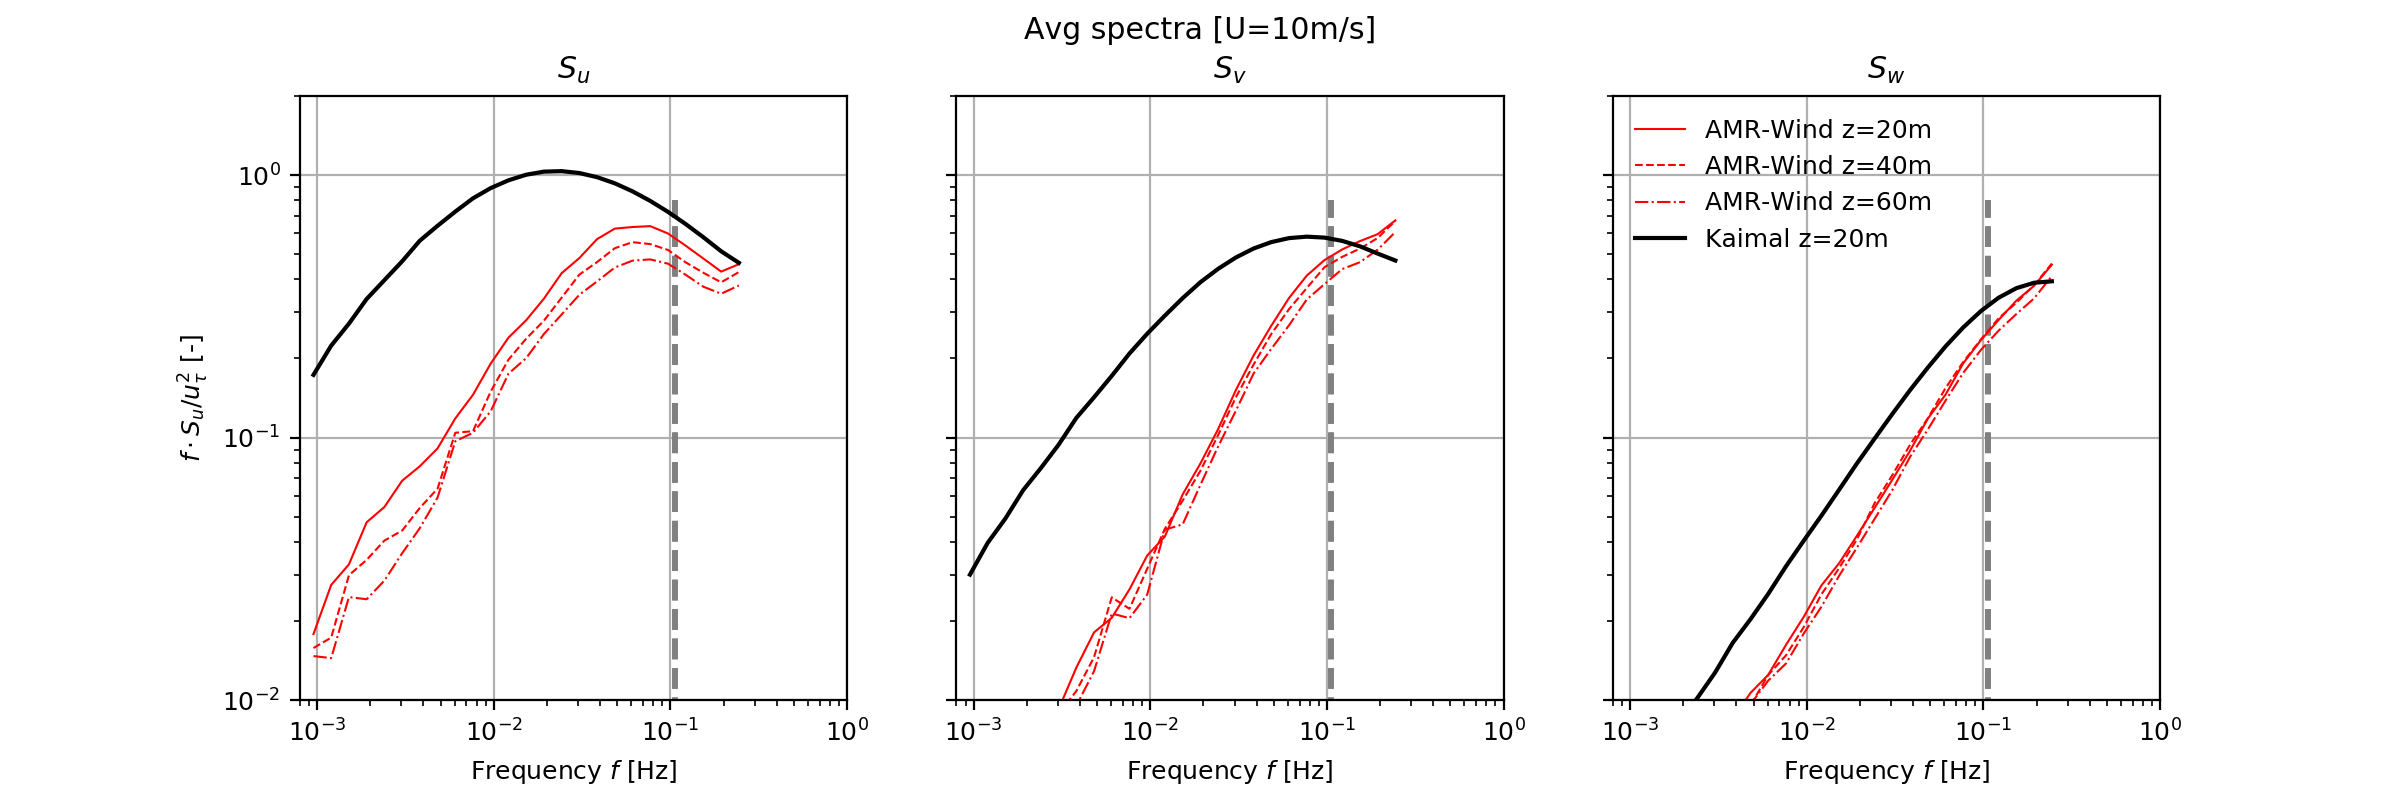
\includegraphics[width=7.0in]{figures/Stable_Spectra_AllZ_10ms.png}\\
  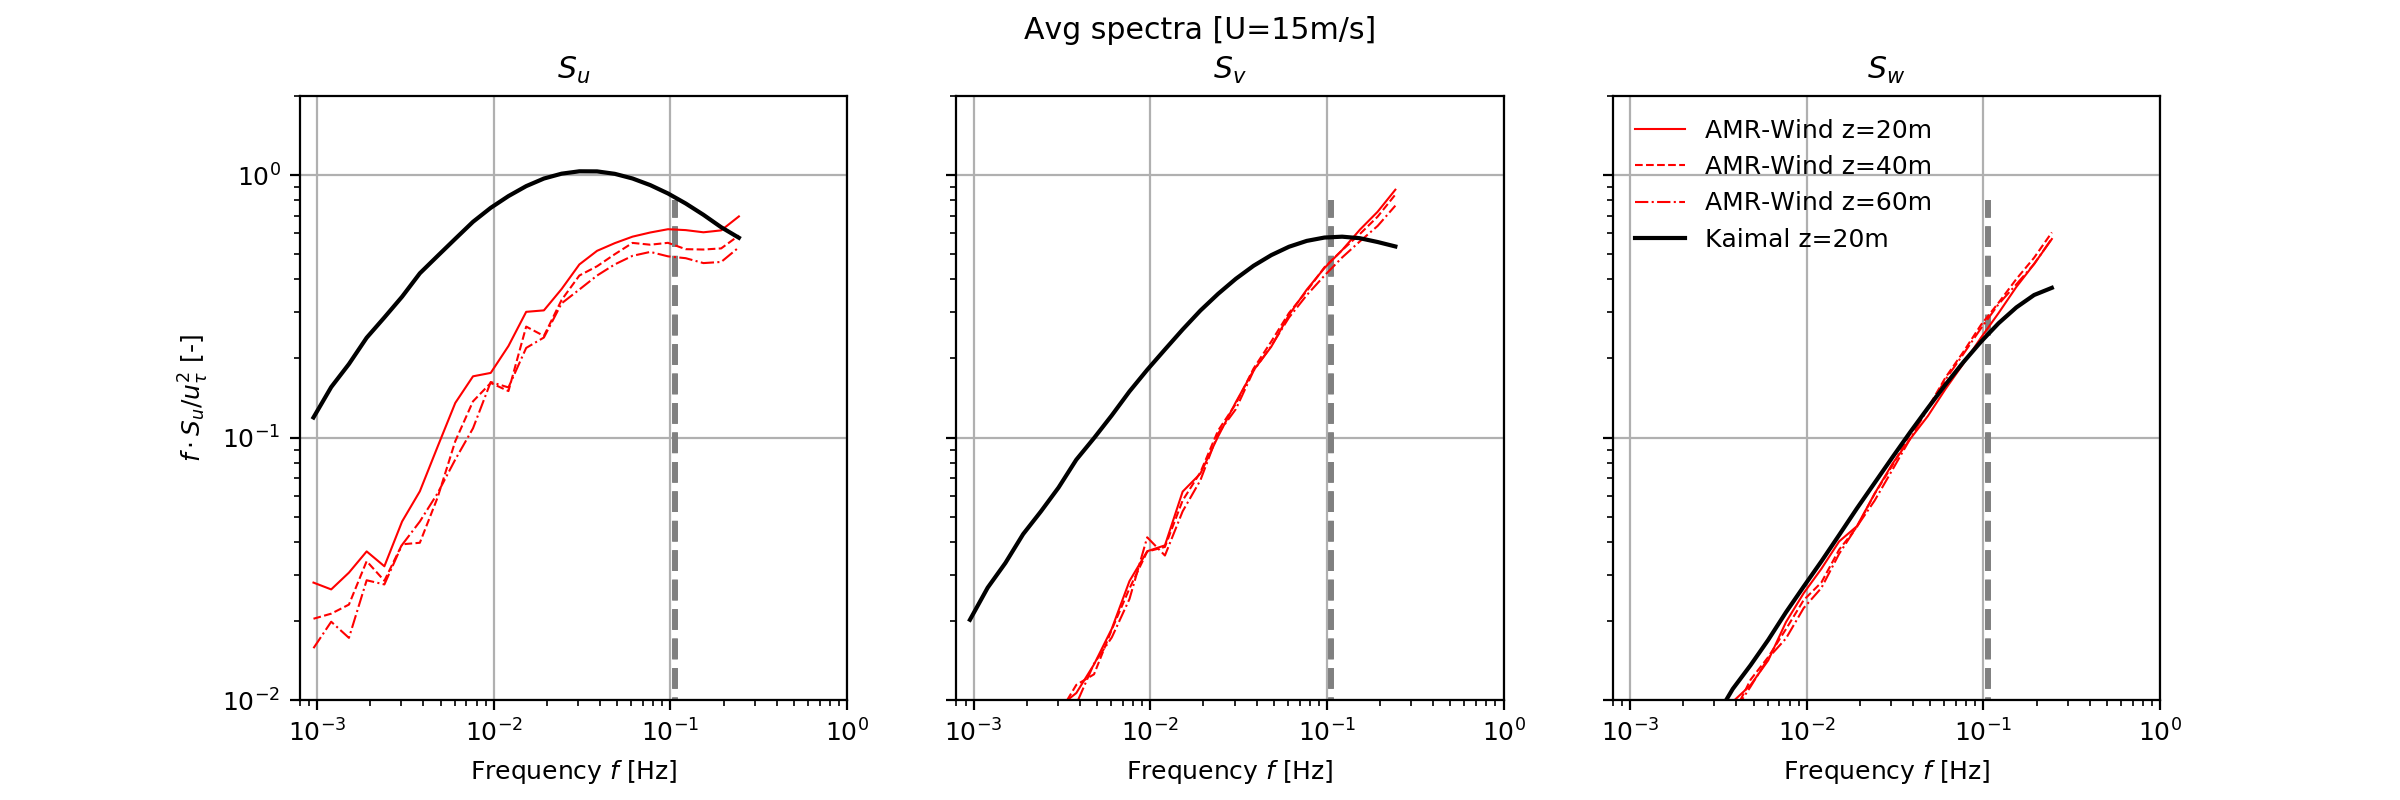
\includegraphics[width=7.0in]{figures/Stable_Spectra_AllZ_15ms.png}
  \caption{Calculation of the wind spectra $S_i$ for LES of stable
    5m/s, 10m/s, and 15m/s cases at z=20m, 40m, and 60m.  The black
    vertical lines correspond to the maximum resolvable frequency
    $f_{max}$ according to equation (\ref{eq:fmax}). }
\end{figure}
%%%%%%%%%%%%%%%%%%%%%%%%%%%%%%%%%%%%%%%%%%%%%%%%%%%%%%%%%%%%%%%%%%%%


\subsubsection{Comparison with neutral and unstable conditions}


%%%%%%%%%%% All stability correlation figure %%%%%%%%%%%%%%%%%%%%
% created in Postprocessing/ABLLength/CompareAll_ABL_Lengthscales.ipynb 
\begin{figure}[hbt!]
  \label{fig:AllStabilityRij}
  \centering
  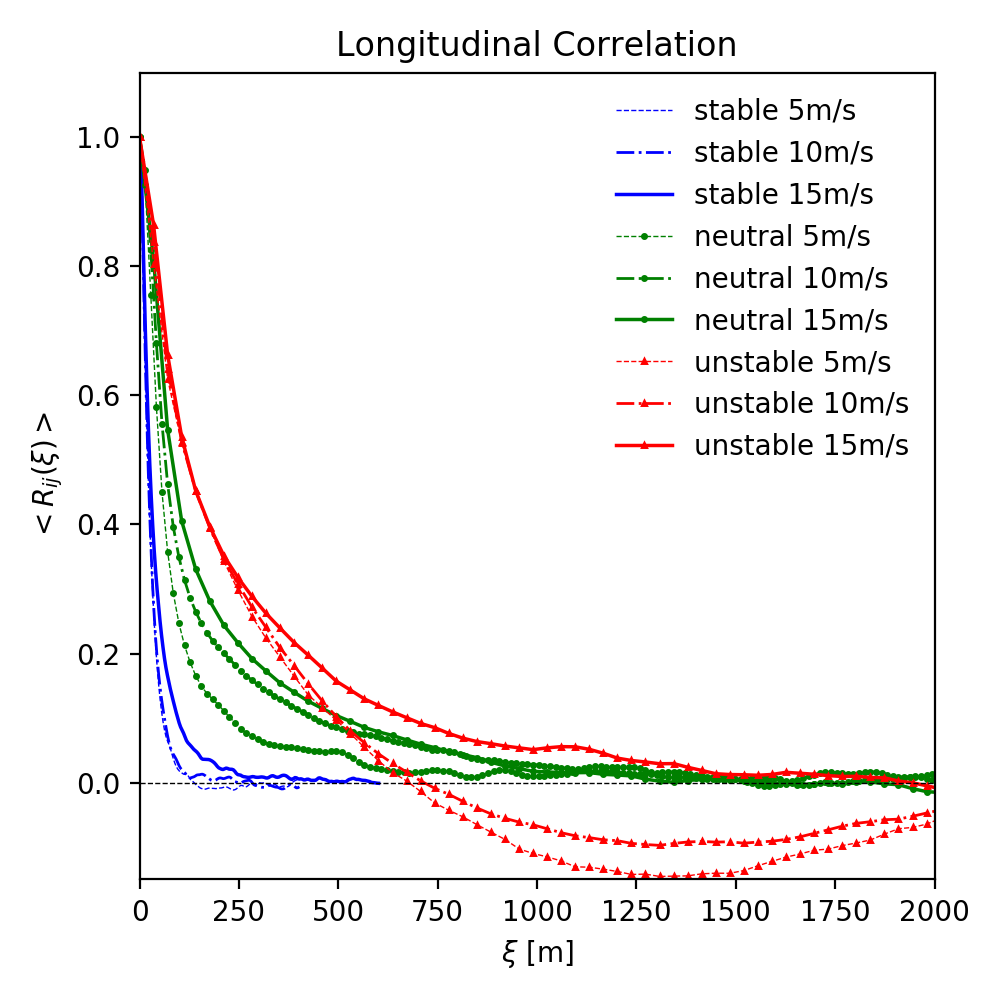
\includegraphics[width=3in]{figures/AllStability_Rij_Longitudinal.png}
  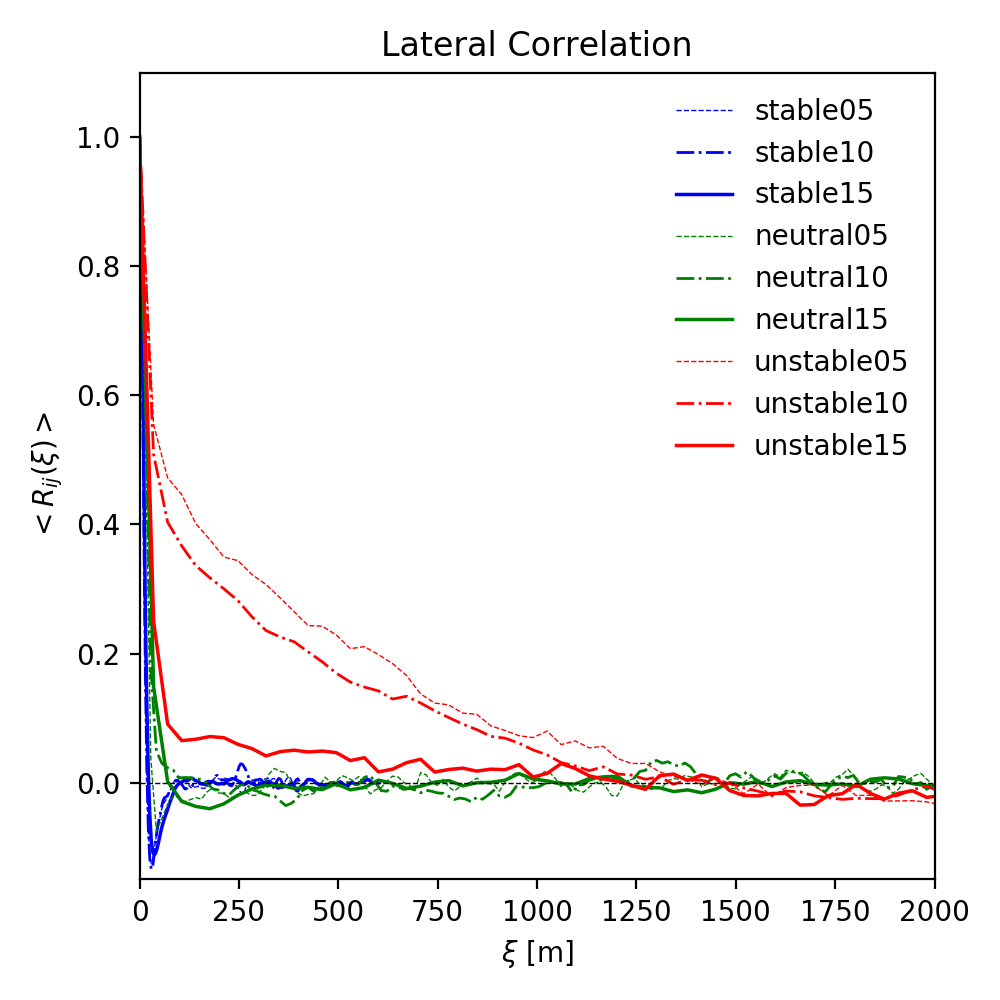
\includegraphics[width=3in]{figures/AllStability_Rij_Lateral.png}
  \caption{Calculation of the averaged longitudinal and lateral
    $R_{ij}(\xi)$ coefficient at $z$=20m for all ABL stability cases.}
\end{figure}
%%%%%%%%%%%%%%%%%%%%%%%%%%%%%%%%%%%%%%%%%%%%%%%%%%%%%%%%%%%%%%%%%%%%

%%%%%%%%%%%%%%% GRID STUDY: INTEGRAL LENGTH %%%%%%%%%%%%%%%%%%%%%%%%%%%%%%%%%%%
\begin{table}
\caption{\label{tab:StabilityStudyLscale} The calculated turbulent
  integral lengthscale for each of atmospheric stabilities} \centering
\begin{tabular}{ccccc}
  \hline
  Stability   & Wind speed & Longitudinal L [m] & Lateral L [m] \\
  \hline
  Stable      &   5 m/s  & 0.0           & 0.0        \\
  Stable      &  10 m/s  & 0.0           & 0.0        \\
  Stable      &  15 m/s  & 0.0           & 0.0        \\
  Neutral     &   5 m/s  & 110.435741    & 15.245327  \\
  Neutral     &  10 m/s  & 165.398368    & 20.634052  \\
  Neutral     &  15 m/s  & 184.081967    & 22.961169  \\
  Unstable    &   5 m/s  & 187.868710    & 270.538753 \\
  Unstable    &  10 m/s  & 177.457502    & 215.027457 \\
  Unstable    &  15 m/s  & 263.475309    & 67.999898  \\
\hline
\end{tabular}
\end{table}
%%%%%%%%%%%%%%%%%%%%%%%%%%%%%%%%%%%%%%%%%%%%%%%%%%%%%%%%%%%%%%%%%%%%
